\chapter{Arquitectura del sistema}
\label{ch:Capitulo 4}

\begin{quote}
  Este capítulo recoge la descripción de la arquitectura del sistema que se ha desarrollado en este trabajo.
\end{quote}

\section{Descripción del sistema}

Como hemos introducido previamente, en este trabajo se va a desarrollar una herramienta que permita trabajar de forma simultánea con datos heterogéneos de distinta procedencia, que posteriormente puedan ser utilizados de forma conjunta en alguna aplicación o problema concreto: en nuestro caso, Food Computing.

\begin{figure}[H]
    \centering
    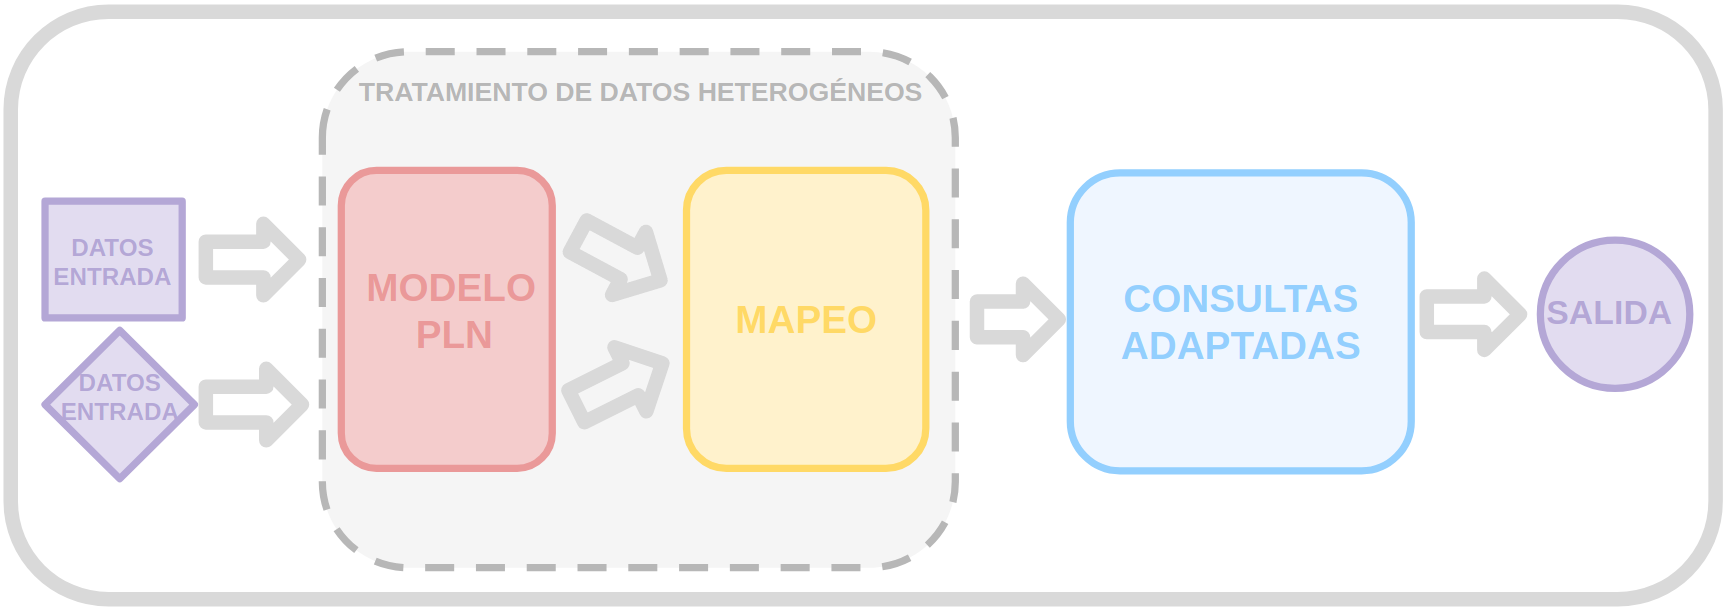
\includegraphics[width=1.0\textwidth]{imagenes/arquitectura/arquitectura-global.png}
    \caption{Arquitectura del sistema}
    \label{fig:arq_1}
\end{figure}

Desde un punto de vista computacional, la resolución de un problema de esta naturaleza se puede modelar como un sistema que funciona en dos fases: una primera fase que se encarga de fusionar los datos de entrada y devolverlos en una estructura que permita poder trabajar con ellos como un todo, y una segunda fase la cual utiliza dicha información fusionada, ya correctamente preprocesada, en el desarrollo de una aplicación que resuelva un problema concreto. Esta idea se puede ver reflejada en la Figura \ref{fig:arq_1}, la cual describe de forma simplificada nuestra propuesta de arquitectura general. En dicha figura se puede observar cómo, a partir de unos datos de entrada heterogéneos entre sí, éstos pasan por un procedimiento que permite trabajar con ellos de forma conjunta (ilustrado en la figura como \textit{Tratamiento de datos heterogéneos}) y poder ser utilizados para llevar a cabo consultas adaptadas a la información una vez fusionada (también apreciable en dicha figura).

\section{Módulos del sistema}

Tal y como se puede apreciar en el esquema de la arquitectura del sistema (ver Figura \ref{fig:arq_1}), las distintas tareas que se llevan a cabo se pueden organizar en módulos independientes, cada uno de ellos ocupándose de una tarea específica que permita cumplir con todos los requisitos del sistema. En dicha figura se pueden apreciar dos primeros módulos, \textit{Modelo de Procesamiento de Lenguaje Natural (PLN)} y \textit{Mapeo}, los cuales se utilizan para el tratamiento con los datos de entrada heterogéneos. Un último módulo denominado \textit{Consultas Adaptadas}, engloba la funcionalidad de un motor de consultas sobre los datos de las distintas fuentes una vez que ya están fusionados.%, representando un único conjunto agregado.

Cada uno de estos módulos es independiente de los demás, y se encarga de una labor específica necesaria para el funcionamiento global del sistema. La funcionalidad de cada uno de ellos, así como su papel en el sistema, se detalla a continuación.

\subsection{Módulo de Procesamiento de Lenguaje Natural}

Este módulo hace referencia al modelo de Procesamiento de Lenguaje Natural (PLN) que se ha implementado para el tratamiento de información textual en este trabajo. Permite obtener una representación de las descripciones textuales de los distintos datos que se introducen como entrada al sistema (ver objetos \textit{Datos entrada} en la Figura \ref{fig:arq_1}). En este punto, se debe tener en cuenta que no hay restricciones previas sobre los datos de entrada más allá de que deban tener descripciones textuales del mismo ámbito para poder llevar a cabo la fusión entre ellos. Por ejemplo, combinar una receta con una base de datos de alimentos a través de las descripciones textuales de los ingredientes de la receta y las de los alimentos de la base de datos de composición nutricional.

Los datos de entrada son procesados en este módulo, para así obtener la representación en el modelo de lenguaje de la descripción textual de cada uno de los datos introducidos. Estos datos pueden ser datos individuales (p.ej., una receta), o un conjunto de ellos (p.ej., colecciones de recetas o bases de datos de alimentos). El componente principal de este módulo, y por el cual se obtienen las representaciones textuales que utiliza el sistema, es un modelo de procesamiento de lenguaje formado por un Word Embedding entrenado en el dominio específico del problema que se pretende resolver. 

En el Capítulo \ref{ch:Capitulo 5} se describe de manera detallada el desarrollo e implementación del modelo de lenguaje. Finalmente, como salida de este módulo, se devuelven las representaciones de las descripciones textuales de los datos que se han proporcionada como entrada al sistema. Las representaciones que se obtienen como salida de este módulo son con las que se trabajará en los módulos restantes que engloban el funcionamiento del sistema. En la Figura \ref{fig:arq_modelo_nlp} se puede ver en mayor detalle el contenido de este módulo. En ella se aprecia el modelo de lenguaje basado en Word Embedding.

\begin{figure}[H]
    \centering
    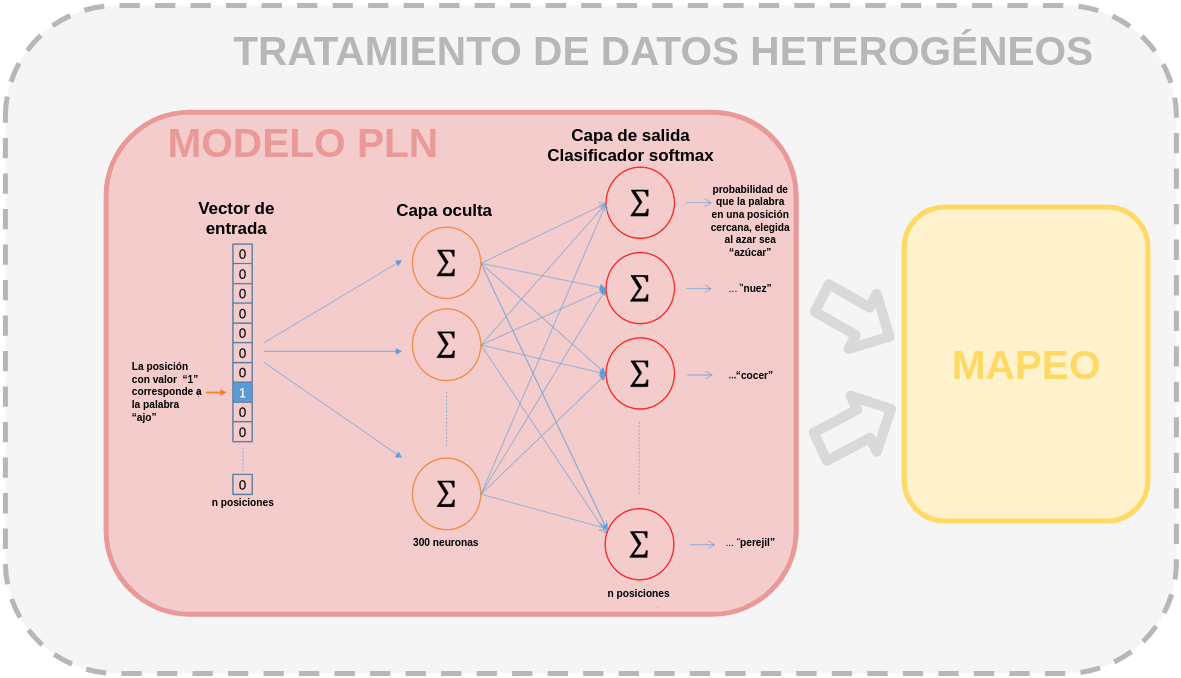
\includegraphics[width=1.0\textwidth]{imagenes/arquitectura/wembedding.png}
    \caption{Arquitectura del sistema: módulo de NLP}
    \label{fig:arq_modelo_nlp}
\end{figure}

\subsection{Módulo de Mapeo}

Este módulo se encarga de identificar las posibles equivalencias entre los datos de entrada, los cuales, como ya se ha mencionado anteriormente, son de naturaleza heterogénea y distinta procedencia. Para ello, se encarga de obtener la mejor correspondencia posible entre los datos proporcionados como entrada al sistema. Este cálculo se realiza en dos pasos:

\begin{enumerate}
    \item En primer lugar se calcula la similitud entre las descripciones textuales de los datos heterogéneos que se han proporcionado. Para ello, se calcula la distancia entre las representaciones que devuelve el módulo de procesamiento del lenguaje de los datos de entrada que se quieren fusionar. Por ejemplo, supongamos que queremos conocer los valores nutricionales de un alimento concreto, y para ello queremos mapear dicho alimento a una base de datos de composición nutricional. En este primer paso, se calcularía la similitud entre el alimento en cuestión y cada uno de los alimentos que se encuentran en la base de datos (los cuales son candidatos a ser el equivalente de dicho alimento en esa base de datos).
    
    \item En segundo y último lugar, se obtiene, de entre todos los posibles candidatos, aquella correspondencia con la que se obtenga la mayor similitud. Volviendo al ejemplo del punto anterior, en este segundo paso nos quedaríamos aquel elemento de la base de datos de composición nutricional cuya similitud con el alimento a fusionar sea máxima.

\end{enumerate}

El funcionamiento que se ha detallado en los dos puntos anteriores se puede ver en la Figura \ref{fig:arq_mapping}, la cual muestra de forma esquematizada las distintas tareas que se abordan en este módulo. Como se puede apreciar en dicha figura, a partir de las representaciones del módulo de procesamiento del lenguaje se establecen correspondencias entre los datos de entrada utilizando el módulo de Mapeo, los cuales permiten trabajar de forma conjunta con los distintos datos que se introducen al sistema.

\begin{figure}[H]
    \centering
    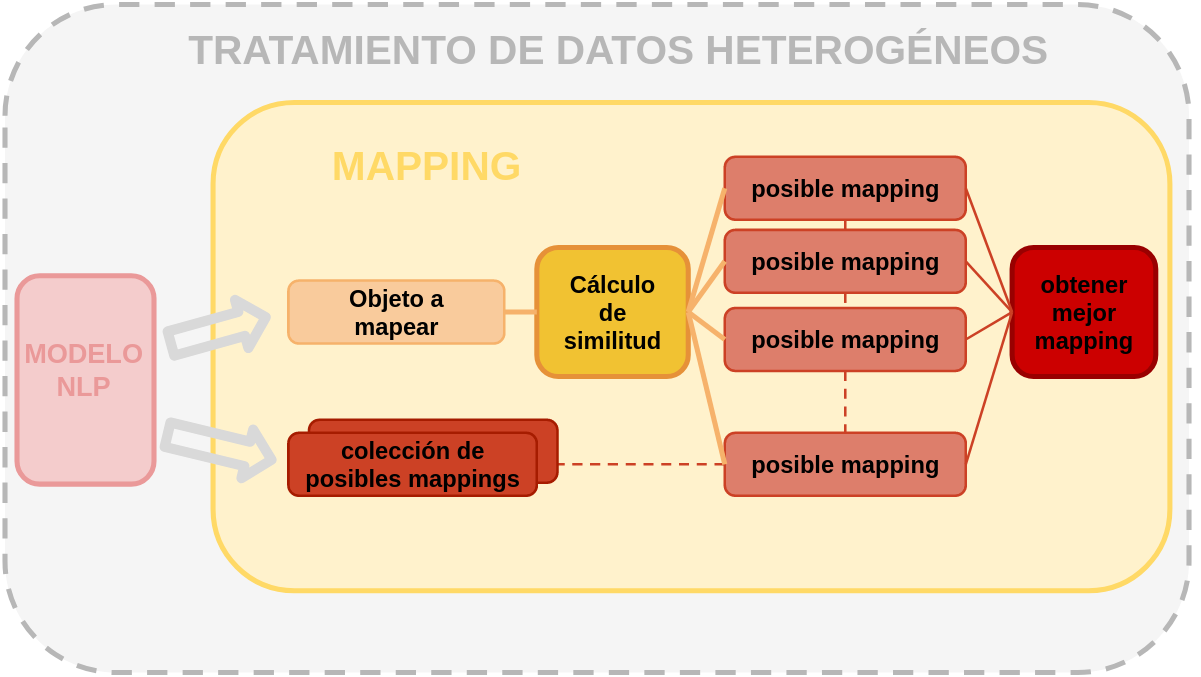
\includegraphics[width=1.0\textwidth]{imagenes/arquitectura/mapping.png}
    \caption{Arquitectura del sistema: módulo de Mapping}
    \label{fig:arq_mapping}
\end{figure}

Debido a la labor general que abarcan tanto este módulo como el de procesamiento de lenguaje, su funcionalidad se puede ver de forma conjunta a más alto nivel, como una única tarea de combinación de información heterogénea llevada a cabo por dos módulos internos independientes. Esta tarea se encarga de establecer las relaciones necesarias entre los datos de entrada para poder trabajar con ellos de forma agregada y así un tercer módulo (en nuestro caso, un módulo de consultas) pueda utilizar dichos datos de forma conjunta. En el Capítulo \ref{ch:Capitulo 6}, se detalla el comportamiento de este módulo.

\subsection{Módulo de Consultas Adaptadas}
A diferencia de los módulos anteriores, los cuales tienen una funcionalidad orientada al tratamiento de las fuentes de datos heterogéneas, la de este último se basa en facilitar la realización de operaciones de consulta que requieran el uso de dichas fuentes de datos de forma simultánea. En otras palabras, a través de este módulo se facilitan los datos, previamente agregados, que resuelvan los requisitos necesarios para el problema en cuestión que se quiera resolver. Estos requisitos dependerán de la tarea específica para la que se quieran utilizar los datos, la cual es independiente tanto de la arquitectura del sistema como del área de aplicación.

\begin{figure}[H]
    \centering
    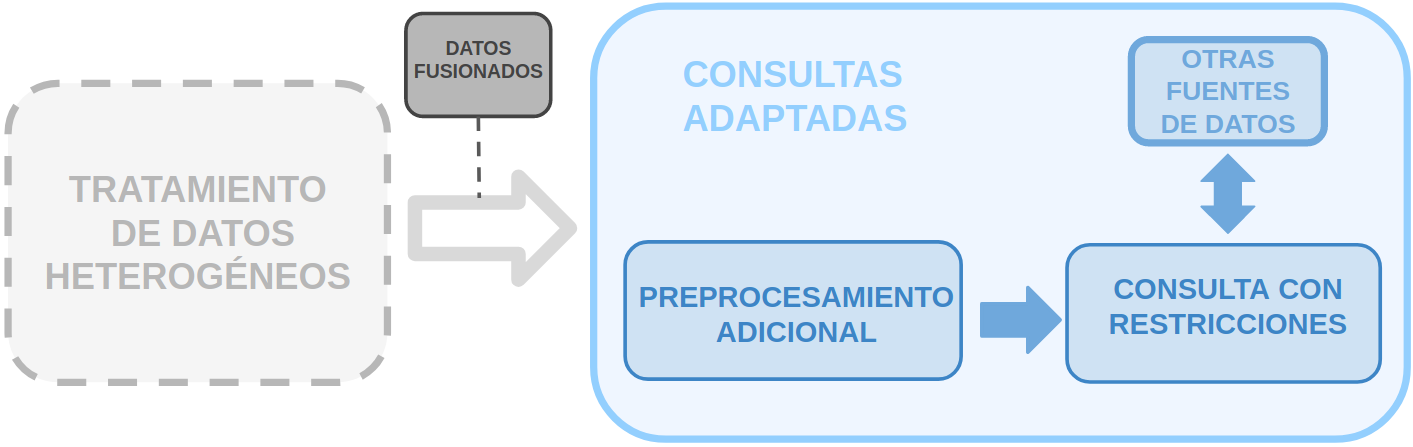
\includegraphics[width=1.0\textwidth]{imagenes/arquitectura/modulo-consulta.png}
    \caption{Arquitectura del sistema: módulo de Consultas Adaptadas}
    \label{fig:arq_application}
\end{figure}

En la Figura \ref{fig:arq_application} se muestra de manera esquematizada la funcionalidad que se implementa en el interior de este módulo. En ella se aprecia cómo se permite obtener la información ya fusionada de manera homogénea por medio de consultas específicas. Estas consultas dependen completamente del problema que se pretende resolver y tal y como se puede ver en dicha figura, aquí pueden incluirse otras bases de datos o algunas tareas adicionales de preprocesamiento para adecuar los datos al uso o tipo de consulta específica llevar a cabo. Este módulo representa el objetivo último del sistema que se ha implementado, y se corresponde con la propia salida del mismo (ver objeto \textit{Salida} en Figura \ref{fig:arq_1}). Su funcionamiento se describe de forma detallada en el Capítulo \ref{ch:Consultas_Adaptadas}.

\section{Sistema para adaptación de dietas en Food Computing}

En este trabajo, se ha implementado una aplicación simple que permita testear el comportamiento y alcance de la herramienta de fusión de datos heterogéneos que se ha desarrollado, probando su funcionamiento en un sistema real como el descrito en los apartados anteriores. Para ello, se ha abordado un problema de gran relevancia en el mundo de la nutrición y el asesoramiento dietético, el cual consiste en aplicar restricciones alimenticias a recetas, adecuando para ello sus ingredientes por otros más idóneos que sí cumplan con dichas restricciones: dada una receta (y sus ingredientes) y una restricción alimenticia concreta, se adaptarán sus ingredientes para que la receta satisfaga las especificaciones proporcionadas. Por ejemplo, una receta con carne podría ser convertida en una receta vegetariana, modificando los ingredientes pertinentes por otros que sí cumplan las restricciones indicadas.

Este sistema se ha implementado como núcleo de una aplicación móvil que gestiona una colección de recetas, permitiendo adaptarlas a una restricción alimenticia concreta seleccionada por el usuario. Para poder abordar esta tarea, se hace uso de la lista de ingredientes correspondiente a la receta en cuestión y de una base de datos de composición de alimentos. Estos datos, de naturaleza claramente heterogénea, necesitan fusionarse para poder conocer las características nutricionales de la receta, y así poder aplicar las restricciones pertinentes. Por ello, se agregan estos datos por medio de la herramienta de fusión de datos heterogéneos, mapeando los ingredientes de la receta con la base de datos de composición nutricional de alimentos de forma que podamos realizar las sustituciones con un respaldo nutricional. Esta secuencia de tareas puede verse en la Figura \ref{fig:arq_application_food_comp}, donde se muestra la arquitectura global del sistema descrito anteriormente, pero ya aplicada al problema en cuestión.

\begin{figure}[H]
    \centering
    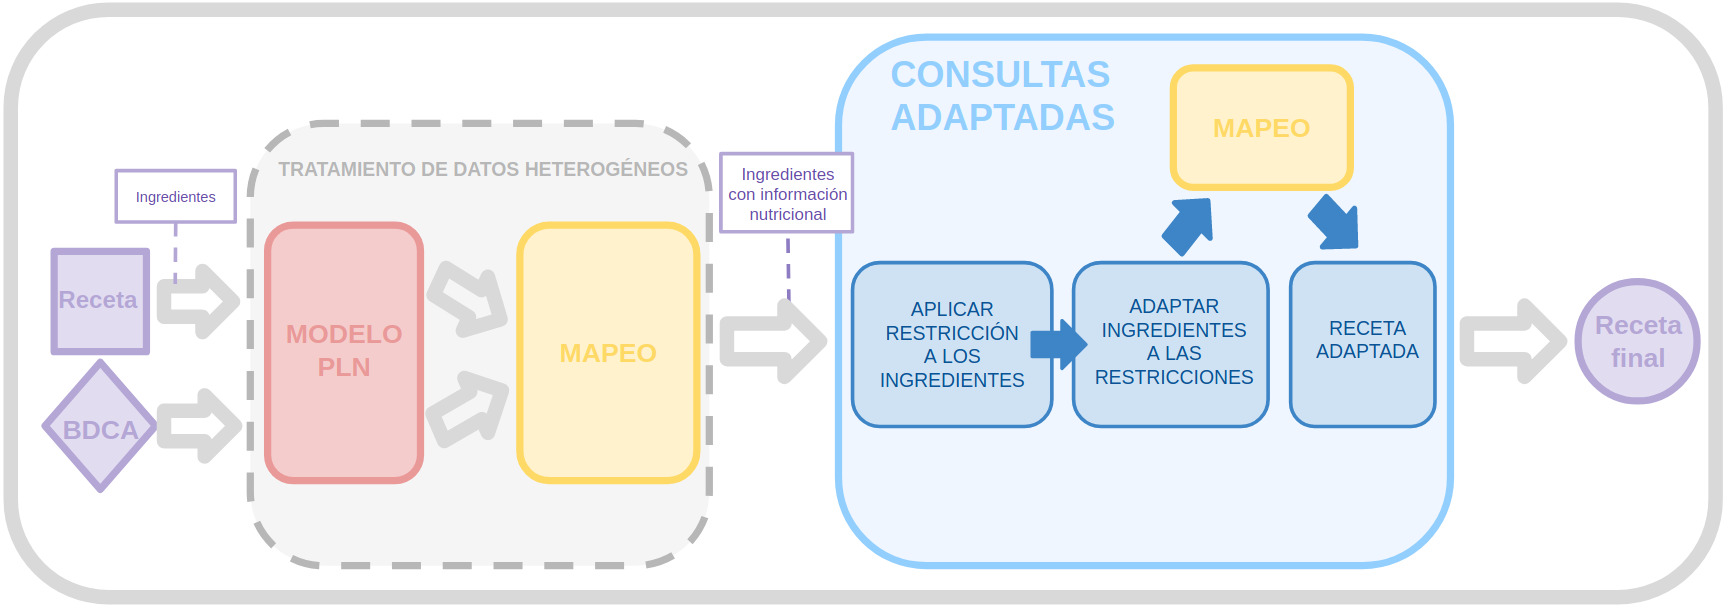
\includegraphics[width=1.0\textwidth]{imagenes/arquitectura/arquitectura-fcomputing.png}
    \caption{Arquitectura del sistema aplicada al problema de adaptación de dietas en Food Computing}
    \label{fig:arq_application_food_comp}
\end{figure}

